\chapter{How I Turned \(-\$20\) Million Into \(\$3.3\) Billion}

This chapter follows a School of Hard Knocks interview with Steven Klubeck, curated by LazyingArt LLC with Video2Book. There is no blackboard in this lecture and no formal mathematical derivation in the usual physics sense. The mathematical payload is instead the structure of a business trajectory: a negative starting point, a claimed multi-billion-dollar exit, a sequence of failures converted into operating knowledge, and repeated rules about trust, capital, brand, and scale.

\section{The Hook: From Millionaire Question to Billion-Dollar Exit}

The lecture begins with a reversal. The interviewer remembers stopping a man in Beverly Hills and asking the standard question: how old were you when you became a millionaire? The answer refuses the premise. Klubeck says, in effect, that the right question is not about being a millionaire. He is a billionaire.

The first numbers arrive quickly. Klubeck identifies the business as hospitality. He owned hotels, says the company operated across \(35\) countries, and says Hilton owns the company today. The sale is described with language that should be kept cautious: the transcript places \(\$2.2\) billion, \(\$3.3\) billion equity value, and enterprise value close together. We should not repair that ambiguity into a cleaner claim than the source gives us.

The quantitative spine is therefore best recorded as a set of interview-backed coordinates:
\begin{align}
W_0 &\approx -\$20\,\text{million},\\
V_{\text{exit}} &\approx \$3.3\,\text{billion},\\
N_{\text{countries}} &= 35,\\
N_{\text{views}} &> 100\,\text{million}.
\end{align}
Here \(W_0\) is not an audited balance-sheet variable. It is the narrated starting point: the negative position the audience already knew from the prior viral clip. Likewise, \(V_{\text{exit}}\) is a compact notation for the value claim in the interview, not a resolved distinction between enterprise value and equity value.

The opening also gives us the chapter's governing question. How does a person move from a broken position to an enterprise that can be sold to one of the largest hotel groups in the world? The transcript does not answer by starting with capital markets. It starts with broken work.

\section{The Broken First Lesson}

The first real origin story is not the famous hotel. It is a shopping center that went badly. Klubeck says he had never built a hotel; he had built shopping centers. One shopping center gave him nearly every problem imaginable: contractors went broke, he paid for lumber twice, he did not understand lien releases, tenants went broke, the economy deteriorated, and an expensive retaining wall appeared outside the plans.

The immediate result was not victory. He says he lost the shopping center, though he did not go broke. But the transcript treats that loss as an education. He had to learn to read plans, understand building, manage surprises, and survive a project when the comfortable abstractions failed.

A useful way to write the mechanism is not as a profit equation but as a state transition:
\begin{equation}
\text{Failed project}
\;\longrightarrow\;
\text{construction literacy}
\;\longrightarrow\;
\text{hotel-building capability}.
\end{equation}

\subsection{Question \& Answer}

\paragraph{Question.}
How can losing the first project still become the asset?

\paragraph{Answer.}
Because the loss did not only remove capital. It produced knowledge that could not be bought cleanly from outside: how plans fail, how contractors fail, how legal releases matter, how costs appear outside the plan, and how to keep working under pressure. In this interview, the shopping center is not a heroic success story. It is the expensive training ground that makes the next asset possible.

We can formalize that idea with a simple capability update. Let \(K_t\) denote operating knowledge at stage \(t\), and let \(L_t\) denote the lessons extracted from a painful project. Then the relevant update is
\begin{equation}
K_{t+1}=K_t+L_t,
\end{equation}
where \(L_t\) is large precisely because the project exposed many failure modes at once. The mistake would be to write only
\[
\text{project loss}=\text{failure}.
\]
The lecture's logic is closer to
\[
\text{project loss}+\text{survival}+\text{learning}
=
\text{future capability}.
\]

\section{Polo Towers: Customer Fit and Defensible Brand}

The next beat is Polo Towers in Las Vegas. Klubeck says he was \(29\) years old and that Polo Towers was the largest hotel-timeshare complex ever built at one time in the world. He says the project was completed on time and on budget, with his father involved because he was working for his father at the time.

The point of the story is not simply that a young operator built a large project. The transcript immediately turns to customer fit. The word ``polo'' could have made the project feel stiff, elite, or old-English. Klubeck says the customer was a big market, so he did not want the project to feel uncomfortable. The brand had to sound aspirational without excluding the buyer.

That gives the first explicit commercial design rule:
\begin{equation}
\text{Good brand}
=
\text{aspiration}
+
\text{customer comfort}
+
\text{defensibility}.
\end{equation}
The last term matters because Ralph Lauren sued over the name. Klubeck says he had marked Polo Towers for hotel, timeshare, and casino, while Ralph Lauren had not. He fought and kept the brand name. The interview uses this as evidence for a broader rule: trademarks, domains, and names are not decorative. They are part of the asset.

\begin{figure}
\centering
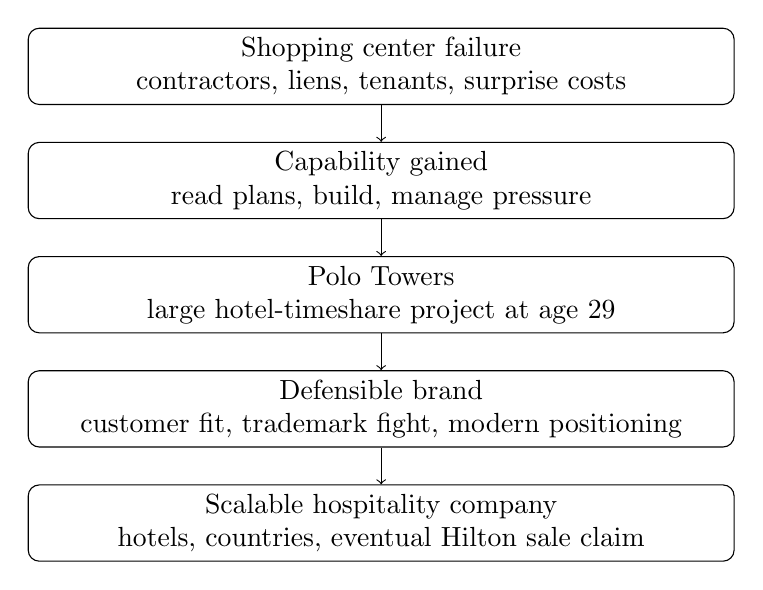
\begin{tikzpicture}[x=1cm,y=1cm]
\node[draw, rounded corners, align=center, text width=.72\linewidth] (a) at (0,0) {Shopping center failure\\contractors, liens, tenants, surprise costs};
\node[draw, rounded corners, align=center, text width=.72\linewidth] (b) at (0,-1.45) {Capability gained\\read plans, build, manage pressure};
\node[draw, rounded corners, align=center, text width=.72\linewidth] (c) at (0,-2.9) {Polo Towers\\large hotel-timeshare project at age \(29\)};
\node[draw, rounded corners, align=center, text width=.72\linewidth] (d) at (0,-4.35) {Defensible brand\\customer fit, trademark fight, modern positioning};
\node[draw, rounded corners, align=center, text width=.72\linewidth] (e) at (0,-5.8) {Scalable hospitality company\\hotels, countries, eventual Hilton sale claim};
\draw[->] (a) -- (b);
\draw[->] (b) -- (c);
\draw[->] (c) -- (d);
\draw[->] (d) -- (e);
\end{tikzpicture}
\caption{A transcript-grounded reconstruction of the path from a failed shopping-center project to a scalable hospitality asset.}
\end{figure}

\section{Brand as a Trust Ledger}

The interview then widens. Klubeck talks about helping create Brand USA, being in charge of tourism for the United States, reporting to the Oval Office, and seeing outsized return on investment. The specific institutional claim should be preserved as an interview claim. The mechanism is more general: he wants the work done, the customers served, and the brand strengthened without pride of authorship.

The later brand discussion makes the rule sharper. The interviewer brings up superheroes as personal brands: figures that stand for and against something. Klubeck answers with integrity. A brand, in this account, takes decades to build and minutes to kill. If someone lies to a customer, trust is broken. If trust is broken, the brand is damaged.

We can model the claim as a ledger, not a logo. Let \(B_t\) denote brand trust at time \(t\), \(S_t\) the service delivered, \(P_t\) the promise made, and \(D_t\) the damage from dishonesty or betrayal. A minimal update rule is
\begin{equation}
B_{t+1}=B_t+\alpha(S_t-P_t)-D_t,
\end{equation}
where \(D_t\) can dominate the equation. The interview's practical version is blunt: do not bust trust.

\subsection{Question \& Answer}

\paragraph{Question.}
Why fire the number-one salesperson if that person produces revenue?

\paragraph{Answer.}
Because the lecture treats revenue and brand damage as different variables. A top salesperson may increase short-term sales, but if that person lies to customers, then \(D_t\) in the brand ledger becomes large. Klubeck says he fired the number-one salesperson in the world because the person created a cancer in the organization. He then claims the company grew by \(20\%\) after the removal.

We should write that as an anecdotal operating claim, not as a controlled causal study:
\begin{equation}
\Delta_{\text{growth}} \approx 20\%
\quad
\text{after removing the salesperson, according to Klubeck.}
\end{equation}
The useful lesson is the structure of the decision. Brand is treated as a compounding asset; dishonesty is treated as a hidden liability.

\section{Operating Range: From Board Level to Making a Bed}

The next movement of the interview is about operating range. Klubeck says that Marriott copied his company's financial presentation, which his CFO found upsetting. Klubeck read it differently: if Marriott copied the deck, that meant the entrepreneurial company had created something worth copying. But he says Marriott could not replicate the company because his organization was nimble.

The phrase he uses is important: a battleship that could move like a speedboat. The reason, in his account, is founder contact with the whole business. He could talk about technology, back-of-house software, tax, accounting, debits, credits, facilities management, and making a bed. The transcript may garble one line as ``I hope write the code,'' likely meaning that he helped write code, but the safe point is operational involvement.

The scale claim later becomes:
\begin{equation}
N_{\text{hotels}}>435,
\qquad
N_{\text{countries}}=35.
\end{equation}
The bridge from one property to hundreds is not described as abstraction away from detail. It is described as standardization of detail. Towels must be placed correctly. Housekeepers must know the standard. Under each bed, he says, there was a card saying that the company cleaned there too. He says he could sweep the floor, cook a meal, serve it, listen to the guest, and clean the table.

The operating rule is:
\begin{equation}
\text{Scale}
\neq
\text{distance from details}.
\end{equation}
In Klubeck's telling, scale comes from turning details into repeatable standards, then making sure the whole team knows that no job is outside the leader's realm of understanding.

\section{Crisis Finance and the Banks}

The interview then turns to 9/11. This is the central risk episode. There were no flights. Hotels had no guests. Klubeck says the cash registers went to zero for everyone. The immediate problem was not branding language but liquidity.

A compact crisis chain is:
\begin{equation}
\text{Flights grounded}
\rightarrow
\text{no guests}
\rightarrow
\text{zero cash registers}
\rightarrow
\text{bank communication}
\rightarrow
\text{additional capital}
\rightarrow
\text{survival}.
\end{equation}
The key behavior is communication. Klubeck says he called his bank every day until the bank asked him to call every three days. He wanted them to know what was happening. He says he had to borrow more money to get through it. The rule he extracts is the same rule as in the brand section: tell the good, the bad, and the ugly.

\subsection{Question \& Answer}

\paragraph{Question.}
What keeps financing alive when revenue stops?

\paragraph{Answer.}
Not optimism. The lecture's answer is credibility. Klubeck says banks trusted him because of capacity, character, and credit: the three C's of banking. In a crisis, the operator cannot promise that conditions are good. What he can do is reduce uncertainty for the lender by telling the truth early and often.

\begin{table}
\centering
\begin{tabular}{lll}
\hline
Criterion & Meaning in the interview & Behavior shown \\
\hline
Capacity & Ability to repay or perform & prior execution and repayment \\
Character & Trustworthiness under stress & candid calls during 9/11 \\
Credit & Financial record and lender confidence & banks view him as good for money \\
\hline
\end{tabular}
\caption{The three C's of banking as used in the interview.}
\end{table}

The working principle is that capital access is path-dependent. If lenders and investors do well with you in one round, they are more likely to return in the next. Klubeck states this as a philosophy: do not try to get the edge on somebody; make sure everyone does well together.

\section{Negotiation, Silence, and the Close}

After the bank discussion, the interview slows down into a negotiation rule. The interviewer recalls that Klubeck once said the first person who talks loses. Klubeck gives a concrete case: he once waited a week, wanting to call and ask whether the other side would do the deal, but he did not pick up the phone. Eventually the call came.

This is a patience rule. The simple algorithm is:
\begin{enumerate}
\item Make the ask.
\item Put the decision in front of the other side.
\item Stop talking.
\item Do not repair the silence with nervous speech.
\item Do not talk past the close after the sale is made.
\end{enumerate}

In notation:
\begin{equation}
T_{\text{wait}}\approx 1\,\text{week}
\end{equation}
for the anecdote, but the rule is not about one week specifically. It is about preserving the force of the close. Once the offer is on the table, additional words can become concessions, apologies, or confusion. Silence is not emptiness; it is part of the bargaining structure.

\section{After the Exit: California as the Next Broken Business}

The final major pivot begins with a contrast. After selling a company for several billion dollars, Klubeck could have chosen leisure. Instead, he says he is running for governor of California. The explanation begins personally: he wanted to live his dream of Beverly Hills, having grown up in the San Fernando Valley. But the argument quickly becomes operational.

He says he interviewed candidates, studied the state, and concluded that California is not merely a state but a country, calling it the fifth largest GDP in the world. Unless separately verified, this should remain framed as a claim made in the interview. He says California is on defense when it should be on offense. He says leaders did not talk to the state's best customers, and that customers fled.

The same business pattern returns:
\begin{align}
N_{\text{interviews}} &> 300,\\
\text{diagnosis} &= \{\text{not affordable},\ \text{not livable},\ \text{not workable}\},\\
\text{repair rule} &= \{\text{respect},\ \text{responsibility},\ \text{results}\}.
\end{align}
This is the same method translated into politics: identify the customer, listen to the customer, locate the broken process, and claim the ability to repair it.

The final analogy is bold and should be kept as Klubeck's framing rather than converted into neutral fact. He says he fixed the most broken businesses, and now sees California as a broken business. Whether one accepts the politics or not, it completes the lecture's internal arc. The same man who learned from a broken shopping center, fixed a broken company, and survived a broken travel market now presents himself as someone willing to enter another broken system.

\section{Summary}

The lecture's structure is a chain of operating claims, each tied to a concrete episode. The first loss teaches construction. Polo Towers turns that knowledge into an asset. Brand becomes a trust ledger. A top salesperson can become a liability if trust is broken. Scale comes from knowing the work at every level, not floating above it. A demand shock like 9/11 tests whether banks believe the operator. Negotiation requires silence after the close. Finally, public service is framed as the same repair problem at a larger scale.

The cleanest mathematical summary is not a formula for wealth but a mechanism:
\begin{equation}
\text{Painful evidence}
\rightarrow
\text{operating discipline}
\rightarrow
\text{trust}
\rightarrow
\text{capital access}
\rightarrow
\text{scale}
\rightarrow
\text{durable value}.
\end{equation}
That is the chapter's source-conscious spine. The numbers give scale, but the interview's repeated lesson is about what makes those numbers possible: learning under pressure, protecting trust, staying close to the customer, and refusing to treat reputation as separate from enterprise value.